\documentclass[8pt]{beamer}
\usetheme{Madrid}
\usefonttheme{serif}

\usepackage{fontspec}
% надёжный шрифт с кириллицей (работает в Overleaf)
\setmainfont{Libertinus Serif}[Ligatures=TeX]
\setsansfont{Libertinus Sans}[Ligatures=TeX]
\newfontfamily\cyrillicfont{Libertinus Serif}
\newfontfamily\cyrillicfontsf{Libertinus Sans}
\usepackage{polyglossia}
\setmainlanguage{russian}
\setotherlanguage{english}

\usepackage{amsmath}
\usepackage{amsfonts}
\usepackage{amssymb}
\usepackage{graphicx}
\usepackage{microtype}

\usepackage{tabularx}
\usepackage{booktabs}

\usepackage{xcolor}
\usepackage{pifont}
\usepackage{tikz}
\newcommand{\plus}{\tikz[baseline=(X.base)] \node[fill=green!65!black, rounded corners=2pt, inner sep=2pt] (X) {\color{white}\ding{51}};}
\newcommand{\minus}{\tikz[baseline=(X.base)] \node[fill=red!70!black,   rounded corners=2pt, inner sep=2pt] (X) {\color{white}\ding{55}};}

\DeclareMathOperator{\sen}{sen}
% \DeclareMathOperator{\tg}{tg}

\setbeamertemplate{caption}[numbered]

% --- Информация о презентации ---
\author[Автор]{Чиняев Владимир Николаевич}
\title{Задача встречи \\ Относительное движение}
\newcommand{\coursename}{Введение в маневрирование КА}
\setbeamertemplate{navigation symbols}{} 
\institute[]{Московский физико технический институт} 
\date{11 ноября 2025 г.} 

\bibliographystyle{apalike}

% --- Кастомная нижняя синяя полоска: курс слева, номер слайда справа ---
\setbeamertemplate{footline}{
  \leavevmode%
  \begin{beamercolorbox}[wd=\paperwidth,ht=2ex,dp=1ex]{palette primary}
    \hspace{0.4cm}\usebeamerfont{footline}\coursename\hfill\usebeamerfont{footline}\insertframenumber\hspace{0.4cm}
  \end{beamercolorbox}%
}

% Чтобы убрать лишние отступы в footer-шрифте (опционально)
\setbeamerfont{footline}{size=\small}

\begin{document}

\begin{frame}
\titlepage
\end{frame}

\begin{frame}{Процесс встречи}
\begin{center}
    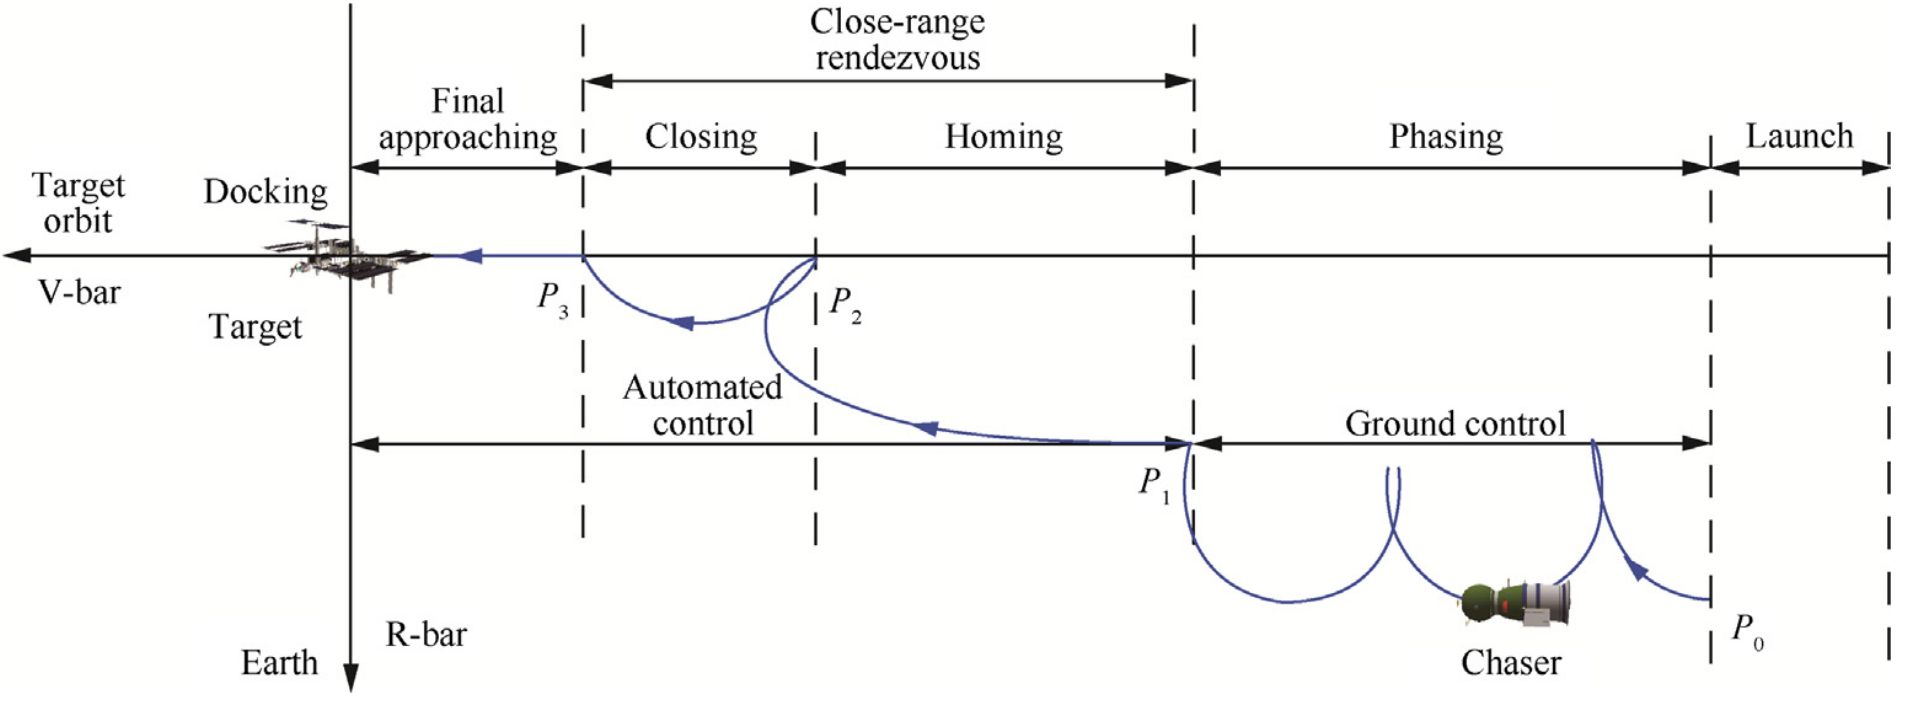
\includegraphics[height=0.45\textheight,keepaspectratio]{images/8/RVD.png}
\end{center}
Процесс встречи делится на несколько фаз:
\begin{align*}
    \textbf{Фазирование} &\longrightarrow \textbf{Встреча короткой продолжительности} \longrightarrow \\ 
    &\longrightarrow \textbf{Заключительный подход} \longrightarrow \textbf{Стыковка}
\end{align*}
В обобщённом сценарии также выделяют \textbf{полёт связанного комплекса} (после стыковки) и \textbf{уход}. \\
Фазу встречи короткой продолжительности обычно делят на этапы \textbf{наведения} (homing) и \textbf{сближения} (closing).
\end{frame}

\begin{frame}{Процесс встречи}
\begin{columns}[T,totalwidth=\textwidth]
  % Левая колонка
  \begin{column}{0.49\textwidth}
    \begin{center}
        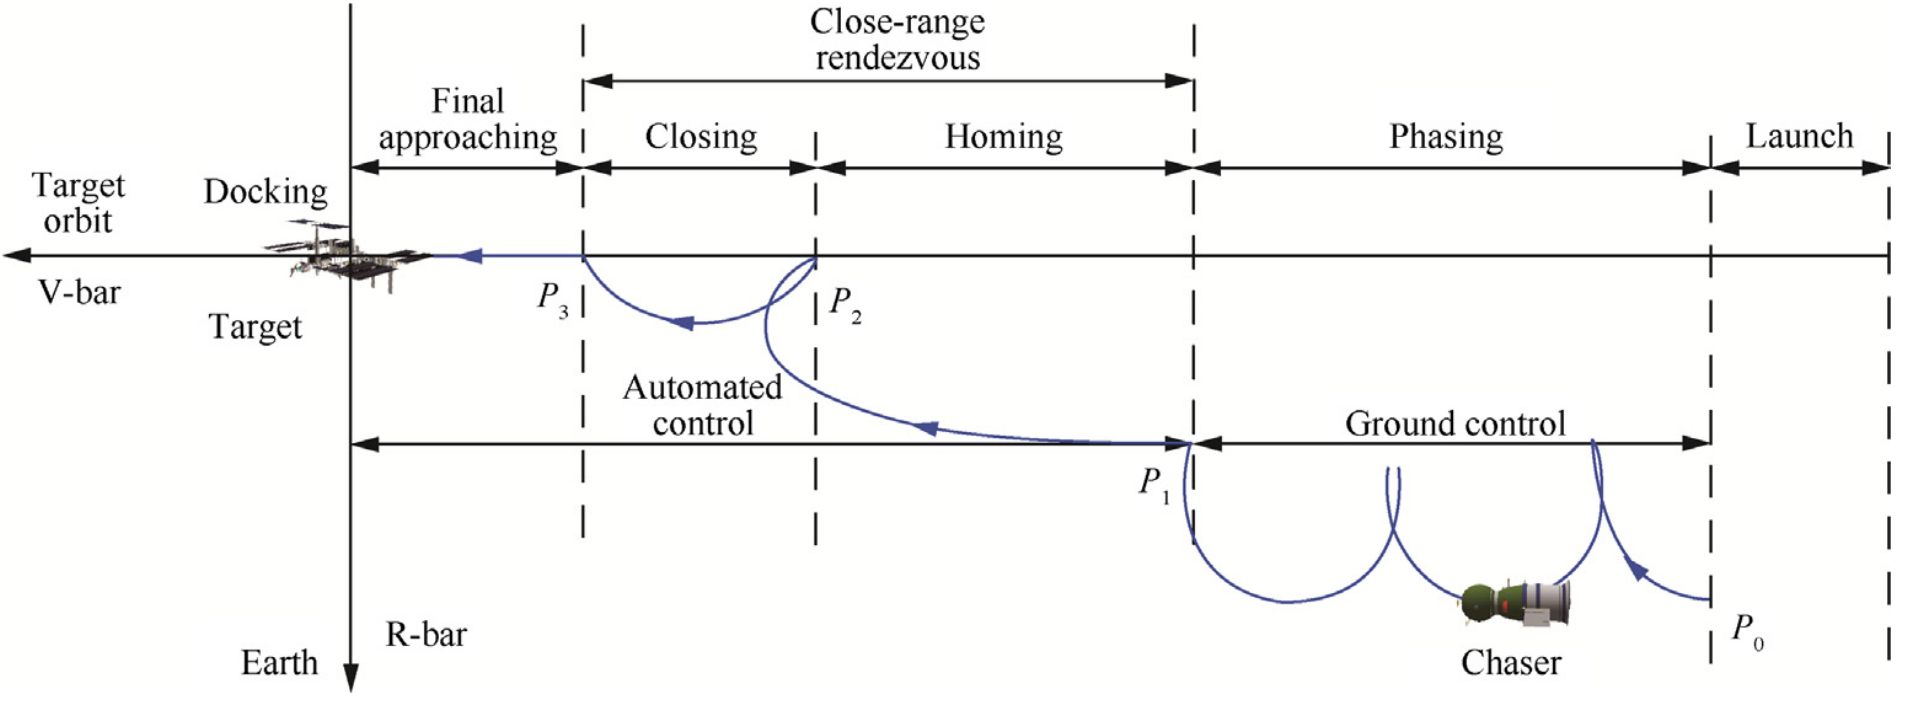
\includegraphics[height=0.25\textheight,keepaspectratio]{images/8/RVD.png}
    \end{center}
    На этапе фазирования КА выполняет ряд манёвров под руководством наземного командно-измерительного комплекса (КИК), чтобы обеспечить захват цели бортовыми навигационными средствами. Главные задачи этапа:
    \begin{itemize}
        \item Выравнивание фазового угла между аппаратами;
        \item Уменьшение рассогласований плоскостей орбит;
        \item Повышение высоты орбиты (при необходимости);
        \item Инициирование относительной навигации.
    \end{itemize}
  \end{column}

  % Правая колонка
  \begin{column}{0.49\textwidth}
    В фазе \textbf{наведения} КА переходит к автономному управлению. Конечная точка этапа - $P_2$, точка на удалении порядка нескольких километров от КА-цели. Основные задачи:
    \begin{itemize}
        \item Выйти на орбиту КА-цели;
        \item Снизить относительную скорость.
    \end{itemize}
    В фазе \textbf{сближения} КА ещё больше уменьшает относительное расстояние и выходит в точку $P_3$ - точку на удалении порядка нескольких сотен метров от КА-цели. 

    Фаза \textbf{заключительного подхода} начинается в $P_3$ и заканчивается касанием/захватом цели. На этом участке стремятся по возможности идти по прямолинейной траектории сближения (линия визирования держится близко к прямой), чтобы выполнить строгие требования стыковки по относительному положению, скорости, ориентации и угловым скоростям. 

    По видам управления: на этапе \textbf{фазирования} преобладают абсолютная навигация и управление; на этапе \textbf{встречи короткой продолжительности} — относительная навигация и управление;
  \end{column}
\end{columns}
\end{frame}

\begin{frame}{Виды навигации}
\begin{columns}[T,totalwidth=\textwidth]
  % Левая колонка
  \begin{column}{0.49\textwidth}
    \begin{center}
        \textbf{Абсолютная навигация}
    \end{center}
    Источники измерений:
    \begin{itemize}
        \item КИК/TT\&C (радиоинтерферометрия, доплер); 
        \item Звёздные датчики; 
        \item Солнечные/магнитные датчики.
    \end{itemize}
    Плюсы:
    \begin{itemize}
        \item Работает на любых дальностях;
        \item Независима от видимости КА-цели;
        \item Хороша для долгих отрезков и больших угловых разносoв.
    \end{itemize}
    Минусы:
    \begin{itemize}
        \item Относительные величины получаются как разность двух оценок $\longrightarrow$ растут коррелированные ошибки и задержки;
        \item На близких дистанциях точности и частоты обновления может не хватать.
    \end{itemize}
  \end{column}

  % Правая колонка
  \begin{column}{0.49\textwidth}
    \begin{center}
        \textbf{Относительная навигация}
    \end{center}
    Источники измерений:
    \begin{itemize}
        \item Лидар/лазерный дальномер;
        \item Оптическое визирование (камера + маркеры);
        \item РЛС ближнего действия;
        \item Ретрорефлектор.
    \end{itemize}
    Плюсы:
    \begin{itemize}
        \item Сантиметровые/субсантиметровые $\Delta r$ и точные углы на малых дистанциях;
    \end{itemize}
    Минусы:
    \begin{itemize}
        \item Требует видимости/маркировки цели и хороших условий освещения;
        \item Диапазон работы ограничен (обычно «километры и ближе»).
    \end{itemize}
  \end{column}
\end{columns}
\end{frame}

\begin{frame}{Уравнения относительной динамики}
Когда расстояние между двумя КА велико, их движение обычно описывают в геоцентрической СК. Когда расстояние между аппаратами достаточно мало, относительное движение, как правило, описывают в орбитальной СК, связанной с КА-целью. Эта СК задаётся так:
\begin{itemize}
    \item Ось z направлена вдоль радиус-вектора от КА-цели к Земле;
    \item Ось y направлена в сторону, противоположную нормали к плоскости орбиты;
    \item Ось x направлена по вектору скорости, замыкая правую тройку.
\end{itemize}
\end{frame}

\begin{frame}{Базовые уравнения относительной динамики}
\begin{columns}[T,totalwidth=\textwidth]
  % Левая колонка
  \begin{column}{0.49\textwidth}
    Система уравнений Клохесси—Уилтшира (Clohessy–Whiltshire, C–W) или уравнения Хилла (Hill):
    \begin{equation*}
        \begin{cases}
            \ddot{x} - 2 \omega \dot{z} = a_x, \\
            \ddot{y} + \omega^2 y = a_y, \\
            \ddot{z} + 2 \omega \dot{x} - 3 \omega^2 z = a_z, 
        \end{cases}
    \end{equation*}
    где $\omega$ - угловая скорость КА-цели; $a_x, a_y, a_z$ - проекции ускорения.

    Система уравнений C-W является системой линейных дифференциальных уравнений, имеет замкнутое аналитическое решение. Относительное движение раскладывается на две независимые части: в плоскости орбиты (плоскость $x-z$) и вне плоскости орбиты ($y$). 
  \end{column}

  % Правая колонка
  \begin{column}{0.49\textwidth}
    Система уравнений C-W получена в следующих приближениях:
    \begin{itemize}
        \item Оба КА движутся по близким околокруговым орбитам;
        \item Относительное расстояние существенно меньше геоцентрического расстояния аппаратов;
        \item Орбитальные возмущения пренебрежимо малы.
    \end{itemize}

    При отсутствии управляющих сил внеплоскостная траектория является тригонометрической волной, а траектория в плоскости орбиты существенно определяется начальными условиями.
  \end{column}
\end{columns}
\end{frame}

\begin{frame}{Улучшенные уравнения относительной динамики}
Система уравнений C-W выводится в предположениях, что 
\begin{itemize}
    \item Аппараты движутся по близким круговым орбитам;
    \item Аппараты движутся в модели двух тел;
    \item Относительное расстояние значительно меньше их геоцентрического расстояния.
\end{itemize}
Кроме того, используются только приближения первого порядка, поэтому члены второго и более высоких порядков по относительным координатам и скоростям отбрасываются. В итоге система C-W корректна лишь для близких по расстоянию и кратковременных (по времени) относительных траекторий. Для описания режимов, не удовлетворяющих этим предпосылкам, требуются уточнения.
\end{frame}

\begin{frame}{Уравнения для больших угловых расстояний}
\begin{columns}[T,totalwidth=\textwidth]
  % Левая колонка
  \begin{column}{0.49\textwidth}
  Система уравнений Баранова:
    \begin{equation*}
        \begin{cases}
            \Delta \dot{r} = \Delta v_r, \\
            \Delta \dot{\theta} = - \omega_0 \frac{\Delta r}{r_0} + \omega_0 \frac{\Delta v_t}{v_0}, \\
            \Delta \dot{z} = \Delta v_z, \\
            \Delta \dot{v}_r = \omega_0^2 \Delta r + 2 \omega_0 \Delta v_t + \Delta a_r, \\
            \Delta \dot{v}_t = -\omega_0 \Delta v_r + \Delta a_t, \\
            \Delta \dot{v}_z = -\omega_0^2 \Delta z + \Delta a_z,
        \end{cases}
    \end{equation*}
    где $r_0$ - средний радиус КА-цели; $\omega_0$ - угловая скорость КА-цели; $v_0$ - орбитальная скорость КА-цели; $\Delta r$, $\Delta \theta$, $\Delta z$ - компоненты относительного положения; $\Delta v_r$, $\Delta v_t$, $\Delta v_z$ - компоненты относительной скорости; $\Delta a_r$, $\Delta a_t$, $\Delta a_z$ - компоненты относительного ускорения.
  \end{column}

  % Правая колонка
  \begin{column}{0.49\textwidth}
    На этапе фазирования разность аргументов широты двух КА, как правило, не мала, и относительное расстояние может быть соизмеримо с геоцентрическим расстоянием. Тогда представление относительного положения и скорости в прямоугольной системе координат становится неэффективным. Баранов предложил описывать такие траектории относительного движения через разность аргументов широты, разность орбитальных радиусов и их производные первого порядка.

    Суть подхода Баранова — формулировать уравнения относительной динамики именно в цилиндрической геоцентрической системе.
  \end{column}
\end{columns}
\end{frame}

\begin{frame}{Уравнения для эллиптических орбит}
\begin{columns}[T,totalwidth=\textwidth]
  % Левая колонка
  \begin{column}{0.49\textwidth}
    Линейные уравнения относительного движения для эллиптических орбит были выведены Цшаунером (Tschauner) и Хемпелем (Hempel) и известны как система T–H. Хотя система T–H линейна, простого замкнутого аналитического решения для неё долго не удавалось найти. 
    \begin{itemize}
        \item Мелтон (Melton) \cite{melton2000time} получил матрицу перехода (STM) для орбит малой эксцентриситетности, опираясь на решение системы C–W и теорию возмущений;
        \item Картер (Carter) \cite{carter1998state} вывел более сложную STM, используя истинную аномалию как независимую переменную;
        \item Яманака (Yamanaka) и Анкерсен (Ankersen) \cite{yamanaka2002new} получили более простую, чем у Картера, STM — также в параметризации по истинной аномалии.
    \end{itemize}
  \end{column}

  % Правая колонка
  \begin{column}{0.49\textwidth}
  Ряд работ уже использует эту STM для алгоритмов наведения на эллиптических орбитах; она основана на следующей системе \cite{yamanaka2002new}:
    \begin{equation*}
        \begin{cases}
            \ddot{x} + k \omega^{3/2} x - 2 \omega \dot{z} - \dot{\omega} z - \omega^2 x = a_x, \\
            \ddot{y} + k \omega^{3/2} y = a_y, \\
            \ddot{z} - 2 k \omega^{3/2} z + 2 \omega \dot{x} + \dot{\omega} x - \omega^2 z = a_z,
        \end{cases}
    \end{equation*}
    где $\mu$ - гравитационный параметр Земли и $k \omega^{3/2} = \mu / r^3$; $r$ - геоцентрическое расстояние до КА-цели.

    Однако при пошаговом прогнозе состояния во времени на каждом шаге требуется решать уравнение Кеплера, и практическая эффективность такой STM всё ещё нуждается в проверке.
  \end{column}
\end{columns}
\end{frame}

\begin{frame}{Уравнения для эллиптических орбит}
\begin{columns}[T,totalwidth=\textwidth]
  % Левая колонка
  \begin{column}{0.49\textwidth}
    По мере увеличения относительного расстояния точность системы C–W падает, поэтому для повышения точности необходимо учитывать квадратичные (второго порядка) члены по относительным координатам и скоростям.
    \begin{itemize}
        \item Лондон (London) \cite{london1963second} выписал систему уравнений с квадратичными членами и получил её приближённое решение на основе решения C–W.
        \item Карлгард (Karlgaard) и Лютце (Lutze) \cite{karlgaard2003second} представили приближённое решение уравнений второго порядка в сферических координатах;
        \item Чжу (Zhu) и Ли (Li) распространили уравнения второго порядка на случай постоянной тяги и рассмотрели случай малой эксцентричности.
    \end{itemize}
  \end{column}

  % Правая колонка
  \begin{column}{0.49\textwidth}
    Широко используемый вариант системы второго порядка выглядит так \cite{london1963second} (здесь показаны характерные квадратичные добавки; $\omega_0, r_0$ относятся к орбите КА-цели):
    \begin{equation*}
        \begin{cases}
            \ddot{x} - 2 \omega_0 \dot{z} + 3 \omega_0^2 \frac{xz}{r_0} = a_x, \\
            \ddot{y} + \omega_0^2 y + 3 \omega_0^2 \frac{yz}{r_0} = a_y, \\
            \ddot{z} + 2 \omega_0 \dot{x} - 3 \omega_0^2 z + \frac{\omega_0^2}{2 r_0} (3 x^2 + 3 y^2 + 6 z^2) = a_z.
        \end{cases}
    \end{equation*}
  \end{column}
\end{columns}
\end{frame}

\begin{frame}{Уравнения с учётом орбитальных возмущений}
\begin{columns}[T,totalwidth=\textwidth]
  % Левая колонка
  \begin{column}{0.49\textwidth}
    В задачах управления спутниковыми группировками (formation flying) разработаны нелинейные системы относительной динамики с учётом возмущений для синтеза конфигураций обладающих устойчивостью или специальной структурой. Например
    \begin{itemize}
        \item Гим (Gim) и Олфренд (Alfriend) \cite{gim2003state} получили сложную STM для эллиптических орбит с учётом возмущений;
        \item Росс (Ross) \cite{ross2003linearized} вывел систему с переменными во времени коэффициентами с учётом возмущения $\text{J}_2$.
    \end{itemize}
    
    Однако такие нелинейные системы громоздки и неудобны для расчёта манёвров. Чтобы обойти это
    \begin{itemize}
        \item Швайгарт (Schweighart) и Седвик (Sedwick) \cite{schweighart2002high} вывели систему с постоянными коэффициентами, добавив к уравнениям C–W долгопериодическое влияние $\text{J}_2$. Cистема имеет замкнутое аналитическое решение и удобна для расчётов;
    \end{itemize}
  \end{column}

  % Правая колонка
  \begin{column}{0.49\textwidth}
    \begin{itemize}
        \item Поллок (Pollock) и соавт. \cite{pollock2011analytical} представили аналитическое решение относительного движения под действием силы Лоренца (электромагнитные возмущения);
        \item Кечичян (Kechichian) \cite{kechichian1992techniques} совместил члены второго порядка с возмущением $\text{J}_2$;
        \item Ямада (Yamada) и соавт. \cite{yamada2012new} добавили $\text{J}_2$ в эллиптическую STM;
        \item Чжан (Zhang) и Чжоу (Zhou) \cite{zhang2010second} получили эллиптическую STM второго порядка с $\text{J}_2$;
    \end{itemize}
    Тем не менее для встречи длительностью один-два витка учёт возмущений редко существенно повышает точность, и поэтому такие уравнения применяются в миссиях встречи заметно реже, чем в задачах построения спутниковых формаций.
  \end{column}
\end{columns}
\end{frame}

\begin{frame}[allowframebreaks]{Источники}
  \begin{thebibliography}{9}

    \bibitem{luo2014survey}
    Luo Y., Zhang J., Tang G. Survey of orbital dynamics and control of space rendezvous //Chinese Journal of Aeronautics. – 2014. – Т. 27. – №. 1. – С. 1-11.

    \bibitem{melton2000time}
    Melton R. G. Time-explicit representation of relative motion between elliptical orbits //Journal of Guidance, Control, and Dynamics. – 2000. – Т. 23. – №. 4. – С. 604-610.

    \bibitem{carter1998state}
    Carter T. E. State transition matrices for terminal rendezvous studies: brief survey and new example //Journal of Guidance, Control, and Dynamics. – 1998. – Т. 21. – №. 1. – С. 148-155.

    \bibitem{yamanaka2002new}
    Yamanaka K., Ankersen F. New state transition matrix for relative motion on an arbitrary elliptical orbit //Journal of guidance, control, and dynamics. – 2002. – Т. 25. – №. 1. – С. 60-66.

    \bibitem{london1963second}
    London H. S. Second approximation to the solution of the rendezvous equations //AIAA journal. – 1963. – Т. 1. – №. 7. – С. 1691-1693.

    \bibitem{karlgaard2003second}
    Karlgaard C. D., Lutze F. H. Second-order relative motion equations //Journal of Guidance, Control, and Dynamics. – 2003. – Т. 26. – №. 1. – С. 41-49.

    \bibitem{gim2003state}
    Gim D. W., Alfriend K. T. State transition matrix of relative motion for the perturbed noncircular reference orbit //Journal of guidance, control, and dynamics. – 2003. – Т. 26. – №. 6. – С. 956-971.

    \bibitem{ross2003linearized}
    Ross I. M. Linearized dynamic equations for spacecraft subject to j perturbations //Journal of Guidance, Control, and Dynamics. – 2003. – Т. 26. – №. 4. – С. 657-659.

    \bibitem{schweighart2002high}
    Schweighart S. A., Sedwick R. J. High-fidelity linearized J model for satellite formation flight //Journal of Guidance, Control, and Dynamics. – 2002. – Т. 25. – №. 6. – С. 1073-1080.

    \bibitem{pollock2011analytical}
    Pollock G. E., Gangestad J. W., Longuski J. M. Analytical solutions for the relative motion of spacecraft subject to Lorentz-force perturbations //Acta Astronautica. – 2011. – Т. 68. – №. 1-2. – С. 204-217.

    \bibitem{kechichian1992techniques}
    Kechichian J. A. Techniques of accurate analytic terminal rendezvous in near-circular orbit //Acta Astronautica. – 1992. – Т. 26. – №. 6. – С. 377-394.

    \bibitem{yamada2012new}
    Yamada K. et al. New state transition matrix for formation flying in J2-perturbed elliptic orbits //Journal of guidance, control, and dynamics. – 2012. – Т. 35. – №. 2. – С. 536-547.

    \bibitem{zhang2010second}
    Zhang G., Zhou D. A second-order solution to the two-point boundary value problem for rendezvous in eccentric orbits //Celestial Mechanics and Dynamical Astronomy. – 2010. – Т. 107. – №. 3. – С. 319-336.
    
  \end{thebibliography}
\end{frame}

\end{document}